\documentclass[prl,aps,twocolumn,showpacs,superscriptaddress,longbibliography]{revtex4-1}

%altaffillsymbol
\usepackage{graphicx}% Include figure files
\usepackage{dcolumn}% Align table columns on decimal point
\usepackage{bm}% bold math
%\usepackage{dsfont}
\usepackage{amssymb,amsmath}
\usepackage{sidecap}
\usepackage{wrapfig}
%\usepackage[bookmarks]{hyperref}
\usepackage{natbib}
%\usepackage{braket}
\usepackage{dsfont}


%\bibliographystyle{apsrev}
%\nofiles
\usepackage{graphicx}
\usepackage{leftidx}
%\usepackage[caption=false]{subfig}
%\usepackage{caption}
%\usepackage{subcaption}
\usepackage{color}

\usepackage{bbold} %This package allows to write the identity symbol

\usepackage{wasysym} % In order to introduce polygon symbols in the text
%aus
%\usepackage[geometry]{ifsym}
%\usepackage{amsbsy}
%\usepackage{bbding}
%\usepackage{universal}
%\usepackage{showkeys}


\usepackage{stackrel}

% color for commenting
\newcommand{\col}[1]{\color{red} #1}
% package for strikethrough
\usepackage{soul,xcolor}
\setstcolor{red}



% ENVIRONMENTS
\newcommand{\be}{\begin{equation}}
\newcommand{\ee}{\end{equation}}
\newcommand{\ba}{\begin{align}}
\newcommand{\ea}{\end{align}}
\newcommand{\sysb}{\left\{\begin{array}}
\newcommand{\syse}{\end{array}\right.}
\newcommand{\baa}{\begin{array}}
\newcommand{\eaa}{\end{array}}
\newcommand{\bs}{\begin{split}}
\newcommand{\es}{\end{split}}

\newcommand{\matb}{\left(\begin{array}}
\newcommand{\mate}{\end{array}\right)}


%VERTICAL SPACES
\newcommand{\vsii}{\vspace{2 mm}}
\newcommand{\vsiii}{\vspace{3 mm}}
\newcommand{\vsiv}{\vspace{4 mm}}

% MEASURES
\newcommand{\ddk}{\int \frac{\rmd^{\left( d-1 \right)}k}{\left( 2\pi \right)^{\left( d-1 \right)}}}
\newcommand{\ddq}{\int \frac{d^{ d-1}q}{\left( 2\pi \right)^{\left( d-1 \right)}}}
\newcommand{\Dq}{\int \mathcal{D}q}
%\newcommand{\dd}[2]{\frac{\rmd^{#1}#2}{\left( 2\pi \right)^{#1 }}}
%\newcommand{\ddr}[2]{\frac{\rm{d}^{#1}#2}{\left( 2\pi \right)^{#1 }}}

% GENERIC SHORTHAND
\newcommand{\mal}{\mathcal}
\newcommand{\rmd}{{\rm{d}}}
\newcommand{\rmD}{{\rm{D}}}
\newcommand{\rme}[1]{{\rm{e}}^{#1}}
\newcommand{\mand}{\quad\text{ and }\quad}
\newcommand{\Dim}[1]{\left[ #1 \right]}
\newcommand{\vphi}{\varphi}
\newcommand{\wh}{\widehat}
\newcommand{\wt}{\widetilde}
\newcommand{\ob}{\mal{O}}
\newcommand{\id}{\mathbb{1}}
\newcommand{\trace}[1]{{\rm tr}\left\{ #1 \right\}}
\newcommand{\order}[1]{O\left( #1 \right)}
\newcommand{\ve}{\varepsilon}
\newcommand{\gh}{\phantom}
\newcommand{\EGamma}[1]{\Gamma \lt #1 \rt}
\newcommand{\ha}{\frac{1}{2}}
\newcommand{\eq}{\, = \,}



% SHORTHANDS SPECIFIC TO THE PRESENT TEXT
\newcommand{\pop}[1]{\hat{n}_{#1}}
\newcommand{\bp}{\mathbf{p}}
\newcommand{\bx}{\mathbf{x}}
\newcommand{\brho}{\bm{\rho}}
\newcommand{\brhoo}{\bm{\rho_0}}
\newcommand{\hsi}{\wh{\sigma}}
\newcommand{\whN}{\wh{N}}
\newcommand{\quadblock}[4]{\matb{c|c} #1 & #2 \\ \hline #3 & #4 \mate}
\newcommand{\bE}{{\bf E}}
\newcommand{\bD}{{\bf D}}
\newcommand{\ce}{\rho}
\newcommand{\sdim}[1]{\lqq #1 \rqq}
\newcommand{\tphi}{\widetilde{\vphi}}
\newcommand{\xp}{x_\perp}
\newcommand{\vth}{\vartheta}
\newcommand{\rmn}{{\rm n}}
\newcommand{\rmr}{{\rm r}}
\newcommand{\hatt}{\hat{t}}
\newcommand{\pp}{{\mathbf{P}}}
\newcommand{\tx}{\tilde{x}}
\newcommand{\ty}{\tilde{y}}



% BRACKETS
\newcommand{\lt}{\left(}
\newcommand{\rt}{\right)}
\newcommand{\lqq}{\left[}
\newcommand{\rqq}{\right]}
\newcommand{\lan}{\left\langle}
\newcommand{\ran}{\right\rangle}
\newcommand{\abs}[1]{\left| #1 \right|}
\newcommand{\eval}[1]{\left.\right|_{ #1 }}
\newcommand{\av}[1]{\lan #1 \ran}
\newcommand{\norm}[1]{\left\| #1 \right\|}
\newcommand{\set}[1]{\left\{  #1  \right\}}



% PAULI MATRICES (SIMBOLS AND MATRIX FORMS)
\newcommand{\sx}{{\sigma^x}}
\newcommand{\sy}{{\sigma^y}}
\newcommand{\sz}{{\sigma^z}}
\newcommand{\sxM}{\matb{cc} 0 & 1 \\ 1 & 0   \mate}
\newcommand{\syM}{\matb{cc} 0 & -i \\ i & 0   \mate}
\newcommand{\szM}{\matb{cc} 1 & 0 \\ 0 & -1   \mate}	
\newcommand{\stx}[1]{\widetilde{\sigma}_{#1}^x}
\newcommand{\sty}[1]{\widetilde{\sigma}_{#1}^y}
\newcommand{\stz}[1]{{\widetilde{\sigma}_{#1}^z}}

% NUMBER SETS
\newcommand{\R}{\mathbb{R}}
\newcommand{\N}{\mathbb{N}}
\newcommand{\Z}{\mathbb{Z}}
\newcommand{\C}{\mathbb{C}}

% QUANTUM MECHANICS
\newcommand{\ket}[1]{\left| #1 \ran}
\newcommand{\bra}[1]{\lan #1 \right|}
\newcommand{\bracket}[2]{\lan #1 \right| \!\left. #2 \ran}
\newcommand{\proj}[1]{\ket{#1} \bra{#1}}
\newcommand{\comm}[2]{\left[ #1, #2 \right]}
\newcommand{\acomm}[2]{\left\{ #1, #2 \right\}}




% TRIGONOMETRIC AND HYPERBOLIC FUNCTIONS
\newcommand{\cosa}[1]{\cos \left(  #1 \right)}
\newcommand{\sina}[1]{\sin \left(  #1 \right)}
\newcommand{\tana}[1]{\tan \left(  #1 \right)}
\newcommand{\cossa}[2]{\cos^{#1} \left(  #2 \right)}
\newcommand{\sinna}[2]{\sin^{#1} \left(  #2 \right)}
\newcommand{\tanna}[2]{\tan^{#1} \left(  #2 \right)}
\newcommand{\tann}[1]{\tan^{#1}}
\newcommand{\cosha}[1]{\cosh \left(  #1 \right)}
\newcommand{\sinha}[1]{\sinh \left(  #1 \right)}
\newcommand{\tanha}[1]{\tanh \left(  #1 \right)}
\newcommand{\cossha}[2]{\cosh^{#1} \left(  #2 \right)}
\newcommand{\sinnha}[2]{\sinh^{#1} \left(  #2 \right)}

% OTHER FUNCTIONS
\newcommand{\loga}[1]{\log \lt #1 \rt}
\newcommand{\lna}[1]{\ln \lt #1 \rt}
\newcommand{\BK}[2]{K_{#1} \lt #2 \rt}
\newcommand{\Prob}{\mathbb{P}}


\newcommand{\nol}{\nonumber \\}


\newcommand{\reff}[1]{(\ref{#1})}
\newcommand{\note}[1]{{\bf \small #1}}

% BOUNDS
\newcommand{\maxx}[2]{\max\limits_{#1}^{} \left\{ #2 \right\}}
\newcommand{\minn}[2]{\min\limits_{#1}^{} \left\{ #2 \right\}}

% LIMITS IN SUMS, INTEGRALS, AND THE LIKE
\newcommand{\prodl}[2]{\prod\limits_{#1}^{#2}}
\newcommand{\suml}[2]{\sum\limits_{#1}^{#2}}
\newcommand{\intl}[2]{\int_{#1}^{#2}}
\newcommand{\bol}[2]{\bigotimes\limits_{#1}^{#2}}
\newcommand{\liml}[1]{\lim\limits_{#1}}



% CORRECTIONS
\newcommand{\change}[1]{\textcolor{blue}{#1}}
\newcommand{\changer}[1]{\textcolor{red}{#1}}
\newcommand{\changeg}[1]{\textcolor{green}{#1}}
\newcommand{\changeb}[1]{\textcolor{blue}{#1}}
\newcommand{\tochange}[1]{\textcolor{magenta}{#1}}
\newcommand{\nochange}[1]{\textcolor{black}{#1}}
\newcommand{\mm}[1]{{\tochange{\footnotesize{\bf (#1)}}}}
\newcommand{\ag}[1]{{\footnotesize \changer{#1}}}
\newcommand{\jm}[1]{{\footnotesize \changeg{#1}}}
\newcommand{\comma}{\quad , \quad}

\newcommand{\dar}{\downarrow}
\newcommand{\uar}{\uparrow}


\newcommand{\transp}{\mathtt{T}}


\newcommand{\ind}{b}
\newcommand{\indd}{c}


\usepackage{amsthm}
\newtheorem{mydef}{Definition}
\newtheorem{prop}{Proposition}
\newtheorem{theorem}{Theorem}


 \newcommand{\up}{\uparrow}
 \newcommand{\uu}{\up\, \up}
 \newcommand{\down}{\downarrow}
 \newcommand{\dd}{\downarrow\, \downarrow}

  \newcommand{\tspace}{\rule{0pt}{2.6ex}}
  \newcommand{\norml}{\textnormal}
  \newcommand{\op}[1]{\mathrm{\hat{#1}}}

\begin{document}

\title{{\color{red} Synthetic lattices, flat bands and localization dynamics in Rydberg quantum simulators in the presence of disorder}}

\author{Maike Ostmann}
\author{Matteo Marcuzzi}
\author{Ji\v{r}\'{i} Min\'{a}\v{r}}
\author{Igor Lesanovsky}
\affiliation{School of Physics and Astronomy, University of Nottingham, Nottingham, NG7 2RD, UK}
\affiliation{Centre for the Mathematics and Theoretical Physics of Quantum Non-equilibrium Systems,
University of Nottingham, Nottingham NG7 2RD, UK}



\begin{abstract}
%We study the physics of Rydberg lattice gases under a so-called facilitation condition, inspired by recent advances in the manipulation of optical tweezer arrays. The facilitation mechanism induces constraints on the connectivity of the Hilbert space, resulting in a highly-simplified structure. When combined with the real space geometry of the tweezer array, it allows the realization of synthetic lattices, where individual sites correspond to many-particle ``Fock'' states. These lattices generically feature the presence of flat bands. We exemplify our construction considering a Rydberg ladder (two close-by linear chains). This maps to a synthetic 1D Lieb lattice, whose flat band supports immobile localized states. We analyse the scaling behaviour of the localization, including anomalous scaling at the band edges, for the correlated disorder imposed by the uncertainty of the atomic positions. Finally, we show how these immobile localized states behave under the influence of increasing disorder, which could in principle be tested in an experiment. 
The dynamics of Rydberg lattice gases under so-called facilitation conditions can be studied on the most recent manifestations of cold atom quantum simulators that employ tailored optical tweezer arrays. Facilitation introduces a constraint which yields a Hilbert space structure that allows the mapping of many-body states onto artificial -- or synthetic -- lattices. These lattices feature in general one or several flat bands and may support immobile localized states. We investigate this for the simple case of a Rydberg ladder. A disordered potential --  imposed by the uncertainty of the atomic positions within the lattice sites -- leads to the localization of the many-body wave function. Moreover, we discuss the experimental preparation of immobile localized many-body states, and how they behave upon the introduction of disorder at different amplitudes.
\end{abstract}
\pacs{}
\maketitle


Over the past few decades, advances in the manipulation of cold and ultra-cold atomic gases made them into a suitable candidate for a versatile quantum simulation platform \cite{Bloch_2008,Bloch_2012}. Indeed, several paradigmatic many-body models have been recreated and studied experimentally, including the Luttinger liquid \cite{hofferberth2007}, Tonks-Girardeau gas \cite{kinoshita2004}, Bose-Hubbard \cite{greiner2002, greiner2003}, and Fermi-Hubbard \cite{Kohl2005}, permitting to directly observe several predicted phenomena, such as quantum revivals \cite{greiner2002_revival}, Lieb-Robinson bounds \cite{cheneau2012}, and topological phase transitions \cite{hadzibabic2006}.


Among many different physical systems apt to act as quantum simulators, ensembles of Rydberg atoms \cite{a_Saffman_RMP_10, Low_2012, Gallagher_1994} stand out for their strong interactions, which are now known to give rise to an intricate phenomenology \cite{Weimer2010, Lan2016, Levi2016, Lan2015, Schempp2014, Schauss_2015, Low2009, Sibalic2016, Carr2013, Marcuzzi2014, Gutierrez2015}. These systems are currently employed for a variety of tasks, such as quantum information processing \cite{Jaksch2000,Weimer_2010,Saffman_2016} and the simulation of quantum spin systems \cite{Labuhn_2015, Schauss_2015}. Several among these instances employ the so-called \emph{anti-blockade} (or \emph{facilitation}) mechanism (see e.g., Refs.~\cite{Ates_2007,Amthor_2010,Garttner_2013,schonleber2014,Lesanovsky_2014,Urvoy_2015,Valado_2016}) to actuate a form of local quantum transport. 

%
%A particular platform, renowned for featuring considerably strong interactions, is given by Rydberg atoms \cite{a_Saffman_RMP_10, Low_2012, Gallagher_1994}. These are atoms whose valence electrons are excited to high-lying orbitals, leading to a noticeably-enhanced polarizability and, consequently, very strong dipole-dipole or van-der-Waals interatomic forces. These systems are now employed for a variety of tasks, ranging from quantum information processing \cite{Jaksch2000,Weimer_2010,Saffman_2016}, to the realization of quantum spin Hamiltonians \cite{Labuhn_2015} and their ground states \cite{Schauss_2015}. A hallmark, characteristic feature of Rydberg atoms is that, even at mesoscopic interatomic distances of a few micrometers, the interaction potentials are still strong enough to shift the atomic levels --- and, therefore, the corresponding transitions --- sufficiently out of resonance with an external electromagnetic field to effectively decouple the atoms from it. This gives rise to a correlated production of excitations leading to a rather rich phenomenology \cite{Weimer2010, Lan2016, Levi2016, Lan2015, Schempp2014, Schauss_2015, Low2009, Sibalic2016, Carr2013, Marcuzzi2014, Gutierrez2015}.

%
%The so-called \emph{facilitation} (or \emph{anti-blockade}) mechanism \cite{Ates_2007,Amthor_2010,Garttner_2013,schonleber2014,Lesanovsky_2014,Urvoy_2015,Valado_2016} emerges upon shining an off-resonant laser on an ensemble of Rydberg atoms. The interactions can then shift the atomic transitions closer to resonance so that atoms at a certain distance from an excited one couple to the laser field and can undergo (de-)excitation. This mechanism therefore translates the global action of the laser on the sample into a local transfer of excitations. This is at the basis of interesting connections to the physics of glasses \cite{Lesanovsky2013} and population dynamics \cite{CPE2017,Marcuzzi2016,Buchhold2017}, but more fundamentally constitutes a form of transport.


In quantum systems, it is well-established that transport can be heavily affected by the presence of quenched disorder, a phenomenon known as Anderson localization \cite{Anderson1958}. In the presence of randomly-distributed impurities in a metal, for example, different paths taken by an electron can interfere destructively, leading to localization , i.e., the electron's wave function is not a Bloch wave extending over the whole system any longer, but spatially localized instead. In one and two dimensions, this effect is so relevant that for arbitrarily small disorder all wavefunctions are localized and transport is effectively impossible \cite{Mott1961,Ishii1973}. Since their first prediction, these effects have been experimentally observed in a range of systems, spanning electron gases \cite{Cutler:1969}, cold atoms \cite{Billy:2008,Roati:2008,Semeghini:2015}, thin films \cite{Liao:2015} and periodically-driven nitrogen molecules \cite{Bitter:2016}. Besides quenched disorder, localized states can also arise in tight-binding models from particular lattice geometries. In these cases, destructive interference leads to the emergence of flat bands. Models with flat bands typically allow the construction of localized eigenstates, and have been experimentally realized with cold atoms \cite{Shen2010}, photonic lattices \cite{Mukherjee2015}, and synthetic solid-state structures \cite{slot2017, drost2017}. When disorder is introduced in such systems, these pre-existing localized states couple to the dispersive, system-spanning ones and start acting like scatterers, inducing a richer phenomenology, such as localization enhancement \cite{Leykam2017}, Anderson transitions in lower-dimensional systems \cite{Bodyfelt2014}, and disorder-induced delocalization \cite{Goda2006}.



In this paper we show that Rydberg quantum simulators offer new capabilities for the study of disorder phenomena in the presence of flat bands. We demonstrate that under facilitation conditions -- when the system parameters are set such that Rydberg states can only be excited next to an already existing excitation -- the Hilbert space acquires a regular lattice structure featuring flat bands. In this picture, the uncertainty of atomic positions translates into a disordered potential on the lattice. Scenarios such as these were previously theoretically explored in \cite{Leykam2017, Bodyfelt2014}. Here we show that they emerge naturally in Rydberg quantum simulators employing optical tweezer arrays. Using the so-called Lieb ladder as an example we predict the scaling of the correlation length, discuss the experimental creation of flat-band eigenstates and their spreading dynamics under the action of different disorder strengths.



% 
%
%In this work, we show how Rydberg gases can also act as quantum simulators for disordered models with flat bands, opening the opportunity to access these phenomena in current experiments. In particular, the advanced control of optical tweezer arrays permits the creation of various lattice geometries \cite{Nogrette_2014, Barredo2017} close to unit filling \cite{Barredo_2016,Endres_2016}. 
% Importantly, techniques allowing for addressing a single atom in such arrays have been developed \cite{Labuhn_2014,Bloch_2016,Greiner_2009,Zwierlein_2015}


\emph{Rydberg facilitation, Hilbert space structure and flat bands---} We start by considering a regular \footnote{We use here the term ``regular'' in a loose sense to denote lattices whose primitive lattice (or, if present, basis) vectors all have the same length.} lattice of $N$ optical tweezers, each loaded with a single Rydberg atom, and with nearest-neighbor distance $R_0$. A laser is shone with a frequency close, up to a detuning $\Delta$, to an atomic transition between the electronic ground state $\ket{\down}$ and a Rydberg level $\ket{\up}$. In a simplified picture, the atoms can thus be described as effective two-level systems. Atoms in the Rydberg state $\ket{\up}$ lying at a distance $d$ from each other interact, if not too close, via an algebraically-decaying potential $V(d) = C_\alpha / d^\alpha$, with $\alpha = 3$ for dipole-dipole interactions and $\alpha = 6$ for van-der-Waals ones. For simplicity, we set $C_\alpha > 0$. Transforming to the frame rotating with the laser frequency and discarding counter-rotating terms (rotating wave approximation), the system can be described by the Hamiltonian [{\color{red} \bf JM: Can we use 1/2 for the interaction here?? Would make it compatible with our PRL paper and also notation I use in the Supplement.}]
%
\begin{align}
 \op{H} = \Omega \, \sum_k^N  \op{\sigma}_x^{(k)} \, + \, \Delta\, \sum_k^N\,\op{n}_k +\,  \,
{\color{red} \frac{1}{2}} \sum_{\substack{k= 1\\ m \ne k}}^N \, V(d_{km}) \, \op{n}_m\, \op{n}_k,
 \label{Eq:Hamil_full}
\end{align}
%
where we set for convenience $\hbar=1$, $\Omega$ is the laser Rabi frequency, $k$ and $m$ are lattice indices, $d_{km}$ denotes the distance between atoms in sites $k$ and $m$, $\op{\sigma}_x^{(k)} = \ket{\up_k} \bra{\down_k} + \ket{\down_k} \bra{\up_k}$ and $\op{n}_k = \proj{\up_k}$. The facilitation (or anti-blockade) condition is obtained by setting $\Delta = -V(R_0)$, so that an isolated excited atom makes its neighbors resonant with the laser. In the following, we assume $\abs{\Delta} \gg \Omega$, so that non-facilitated atoms are sufficiently off-resonant to neglect their excitation. Furthermore, denoting by $R_1$ the distance between next-nearest neighbors, we set $V(R_1) \gg \Omega$ as well. This last condition implies that an isolated excitation can facilitate the production of another on a neighboring site, but no additional one can then be produced in the neighborhood, as the process is energetically suppressed. For example, in one dimension $\abs{\bra{\up \up \up} \rme{-iHt} \ket{\up \up \down}}^2 \sim O((\Omega / V(R_1))^2)$. In the following, we neglect these transitions, effectively splitting the Hilbert space into subspaces separated by energy scales $\gg \Omega$ . Each subspace comprises a set of quasi-resonant states separated by scales $\sim O(\Omega)$ (see Ref.~\cite{a_Marcuzzi_PRL_17} for more details on this structure). From a simple perspective, this means that a single excitation can at most produce one more in the neighborhood, after which either the former facilitates the de-excitation of the latter, or vice versa. Starting from a state with a single excitation, the relevant Hilbert subspace will consist of all states with either a single excitation or a single pair of excitations on neighboring sites. This draws a lattice structure in the Hilbert space which closely resembles the original geometry of the tweezers, according to the following basic rules, sketched in Fig.~\ref{Fig:flat_band_lattices} for a few planar examples:  
\begin{figure}
% 	    

	      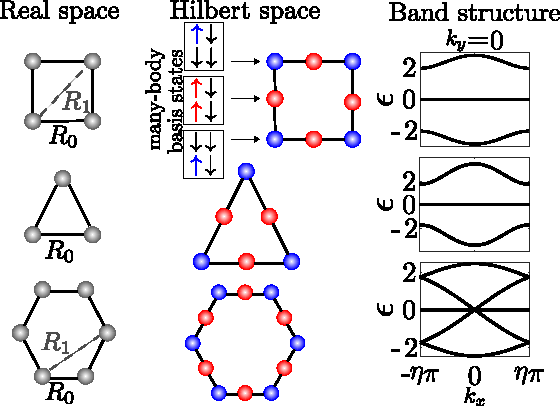
\includegraphics[width=0.5\textwidth]{graphics/lattices_real_hilbert_bands.pdf}

    %
		\caption{
		    First column: geometry of a square, a triangular, and a hexagonal lattice 
		    in real space. The blue spheres give the position of the Rydberg atoms and
		    the lines the interaction between neighboring atoms. Second column: respective lattices in {\color{red} the Hilbert space under
		    the facilitation condition $\Delta = -V(R_0)$.} The blue dots represent the main state with a single excitation while the red spheres
		    are intermediate state corresponding to a single pair of neighboring excitation.
		    Third column: two cuts of the band structure for each lattice geometries at $k_y= 0$ (left) and $k_y = \pi$ (right).
		    The green bands are the flat bands of the respective lattice. The red and blue bands are the dispersive bands of the system
		    (different colors for easier readability).
		    %
                    }
  
	\label{Fig:flat_band_lattices}
\end{figure} 
%%
%%
%%
(i) in the original lattice structure, draw the links joining nearest neighbors; (ii) each site can now be identified with the state having a single excitation on that site. This exhausts all ``one-excitation'' states in the subspace; (iii) each ``pair'' state can be straightforwardly associated to the link joining the two excited atoms; hence, place an additional site in the midpoint of each link and associate it with the corresponding ``pair'' state. The links in this new-found structure now effectively represent pair of states connected by the Hamiltonian, which can be therefore seen as a tight-binding model on a generalised lattice. In the case of a square lattice, the new structure (see Fig.~\ref{Fig:flat_band_lattices}) is called \emph{Lieb lattice} and is known to feature a flat band and two dispersive ones which meet with a cone-like structure at the edges of the first Brillouin zone. However, this construction is general and can be extended to any kind of ``regular'' lattice. Most of these structures will support flat bands as well: It can be shown \cite{SM} that, calling $n_1$ ($n_2$) the number of one-excitation (pair) states in a unit cell, the number of flat bands $n_{\rm flat}$ must be $\geq \abs{n_1 - n_2}$. For the examples of Fig.~\ref{Fig:flat_band_lattices}, {\color{red} the square, triangular and honeycomb lattices have $(n_1,n_2,n_{\rm flat}) = (1,2,1)$, $(1,3,2)$ and $(2,3,1)$ respectively.} These flat bands constitute extensively-degenerate eigenspaces of the Hamiltonian; as such, it is often possible to recombine the usual (plane-wave-like) Bloch solutions to form a set of localised eigenstates. 

\emph{Disorder---} Disorder enters the picture through the uncertainty in the atomic positions: the optical tweezers are not, in fact, infinitely narrow and there is an intrinsic uncertainty in the atomic positions. Due to the noticeable amplitude of the interaction potential $V(d)$, even small displacements from the centre of the traps can significantly shift the atomic transitions off resonance from the laser frequency, thereby hindering the facilitation mechanism, as studied e.g.~in Ref.~\cite{a_Marcuzzi_PRL_17}. In fact, the interaction potential seen by an atom at a distance $R = R_0 + \delta R$ from an excitation will be $V(R) = V(R_0 + \delta R) \equiv V(R_0) + \delta V$; note that, since $V(R) >0$, $\delta V > - V(R_0)$, i.e.~the energy shifts are only defined on a domain $[-V(R_0), +\infty)$. At small disorder ($\delta R \ll R_0$) they can be approximated by $\delta V \approx -\alpha C_\alpha / R_0^{\alpha + 1} \delta R$. These energy shifts are random and only affect pair states, creating a disordered potential landscape over the pair (red) sites in Fig.~\ref{Fig:flat_band_lattices}. The single-excitation (blue) sites' energy remains unvaried instead, which in particular implies that any eigenstates of the tight-binding Hamiltonian which exclusively have component on these sites will be unaffected by disorder, and remain eigenstate of the disordered Hamiltonian at the same energy for any random realization. Note, however, that for the Hilbert space structure to be maintained, the disorder strength cannot exceed the scale of energetic suppression fixed before, i.e.~$\delta V \ll V(R_1)$. 

In order to characterize the disorder, we denote by $\omega$ the optical trapping frequency (assumed hereafter to be isotropic in space), by $m$ the atomic mass and by $T$ the temperature. The probability distribution of a trapped atom can then be approximately described as a Gaussian of width $\sigma$ around the trap centre. We require now that (I) $k_B T \gg \hbar \omega$: this implies that one can use the semiclassical estimate $\sigma \approx \sqrt{k_B T / m\omega^2}$ and moreover that the thermal de Broglie wavelength of the atom is much smaller than the distribution width. In other words, the atom can be approximately considered localized somewhere within the trap according to a classical probability distribution. (II) $\omega \Delta t \ll 1$, with $\Delta t$ the duration of an experiment: this ensures that the atoms will not appreciably move from their positions in this time frame and thus the disorder is quenched. (III) $\Omega \gg \omega$, or in other words the dynamics of the internal degrees of freedom is much faster than the one of the kinetic ones, so that within an experiment one can probe the action of the disordered Hamiltonian on the system while keeping the disorder quenched (i.e.~fixed). The properties of the probability distribution of energy shifts are discussed in \cite{SM}; here we just remark that amplitudes of shifts over different pair sites are not independent, but weakly correlated.


%As pointed out in Ref.~\cite{a_Marcuzzi_PRL_17}, while the positions of the atoms are picked from independent Gaussian distributions, the energy shifts depend on them via the distances $D_{km}$. This produces a correlated distribution $P(\delta V_{km} ,\, \delta V_{m l}) \neq P(\delta V_{km}) P(\delta V_{ml})$. 
%The correlated nature of the distribution of energy shifts can also be inferred from the triangular inequality: since $D_{km} + D_{ml} \geq D_{kl}$ then, using the approximate expression for $\delta V \ll V(R_0)$ shown above one finds $\delta V_{kl} \geq \delta V_{km} + \delta V_{ml} - \alpha V(R_0)$. For weak disorder, this constraint is satisfied most of the times (since $\delta V \geq - V(R_0)$ by construction) which suggests that these correlations do not play any major role. 
%A more detailed discussion of the properties of the probability distribution of energy shifts can be found in \cite{SM}; here we just remark that this distribution is fat-tailed, i.e.~it has no well-defined moments; however, for weak noise its algebraically-decaying tails are suppressed to a point where they could not be probed in any reasonable simulation or experiment.


\emph{Disordered Lieb ladder---} In the remainder of our discussion, we shall focus on a ladder configuration, i.e.~a quasi-one-dimensional lattice formed by placing two linear chains parallel to each other at a lattice spacing distance $R_0$. For this example, the artificial lattice (corresponding to the ``1D Lieb lattice'' case of Ref.~\cite{Leykam2017}) in the Hilbert space is sketched in Fig.~\ref{Fig:decoupling}(a). The unit cell consists of five sites with $n_1 = 2$ and $n_2 = 3$ and the band structure features one zero-energy flat and four dispersive bands grouped in two pairs of opposites (panel (d)). 
%%%
%%%
%
\begin{figure}
% 	    

	      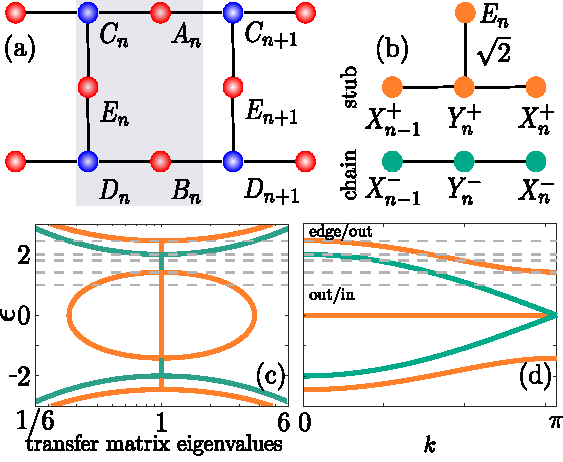
\includegraphics[width=0.5\textwidth]{graphics/decoupling.pdf}

    %
		\caption{Hilbert space structure and spectrum in the absence of disorder. (a) One dimensional Lieb ladder. Blue spheres correspond to one-excitation states while red spheres represent pair states. We introduce a convenient notation for the five sites $A_n$, $B_n$, $C_n$, $D_n$, $E_n$ in the $n$-th unit cell. (b) A change of basis -- the so-called ``detangling'' \cite{a_Flach_EPL_14,Leykam2017} -- maps the Lieb ladder onto two decoupled chains. The $\sqrt{2}$ factor denotes that the hopping amplitude on the vertical link of each unit cell is amplified by that same amount.
		     (c) Eigenvalues of the transfer matrix in loglinear scale \mm{Too few ticks on the horizontal axis, and $0$ may cause confusion}.
		     The dotted lines corresponds to the energies $\epsilon = \{0,1, \sqrt 2, 1.8, 2, \sqrt 6\}$ at which the scaling of the localization lengths is investigated in Fig.~\ref{Fig:2D_loc_length}.
                    (d) Band structure of the Lieb ladder. The bands corresponding to the stub lattice are given in red and bands of the ordinary 1D chain are shown in blue.
                    }
  
	\label{Fig:decoupling}
\end{figure}  
%
%
%%%
%%%
%Via an appropriate change of basis (``detangling transformation'' \cite{a_Flach_EPL_14,Leykam2017}) this Lieb ladder can be mapped onto two uncoupled one-dimensional lattices (see Fig.~\ref{Fig:decoupling}(b)), a chain (in blue, supporting the two innermost dispersive bands) and a stub lattice (in red, supporting the flat and two outermost dispersive bands) \cite{SM}.


%Via a detangling transformation \cite{a_Flach_EPL_14,Leykam2017} this lattice (before the introduction of disorder) can be mapped onto a pair of disjoint ones (see Fig.~\ref{Fig:decoupling}(b)), a chain (in blue, supporting the two innermost dispersive bands) and a stub lattice (in red, supporting the flat and two outermost dispersive bands) \cite{SM}. The states of the flat band can be classified into a macroscopic set of localized ones (of the form $(\ket{A_n} + \ket{B_n} - \ket{E_n} - \ket{E_{n+1}})$) with support exclusively on pair sites plus an extended one (of the form $\sum_n (-1)^n (\ket{C_n} - \ket{D_n})$) with support exclusively on single-excitation sites. The latter is insensitive to the disorder and survives unaffected to its introduction. 

%The Lieb ladder in the presence of disorder is a paradigmatic system for the exploration of disorder phenomena in the presence of flat bands. Moreover, it has been attractive substantial interest in the context of correlated and fat-tailed disorder distributions [PLEASE ADAPT, BUT I THINK YOU GET THE IDEA BEHIND MAKING IT SOUND MORE EXCITING/IMPORTANT]. 
%
%In the Rydberg quantum simulator the situation is made more complex by the fact that disorder is not present on all sites but only the ones that correspond to many-body states containing two adjacent Rydberg atoms (Fig. 1).

This Lieb ladder constitutes one of the simplest examples where flat bands produce a non-trivial interplay with the on-site disorder \cite{Leykam2017}. In a Rydberg quantum simulator, however, the underlying structure is made more complex by the fact that disorder only appears on pair states. In other words, all the blue sites in Fig.~\ref{Fig:flat_band_lattices}(a) are, by construction, unaffected by it.
% in the presence of disorder constitutes one of the simplest examples of systems with a non-trivial interplay between the on-site disorder
%A similar model was studied in Ref.~\cite{Leykam2017}, where however the disorder was generated independently on each site. 
In order to establish a connection with the results of Ref.~\cite{Leykam2017} we study in the following the scaling behaviour of the \emph{localization length} $\xi$ at small disorder. 
%assess how much the localization properties may be affected by having no disorder on half of the lattice sites, we start by performing an analogous study of the scaling properties of the \emph{localization length} $\xi$ at small disorder.
This quantity describes, at fixed energy $\epsilon$, the exponential envelope of eigenstates of the disordered Hamiltonian; in other words, wave functions are peaked and mostly concentrated in a specific area of the lattice and decay as $\rme{-x/\xi}$ with the distance $r$ from it (in the longitudinal direction).
%
Via an appropriate change of basis (``detangling transformation'' \cite{a_Flach_EPL_14,Leykam2017}) this Lieb ladder can be mapped onto two uncoupled one-dimensional lattices (see Fig.~\ref{Fig:decoupling}(b)), a chain (in blue, supporting the two innermost dispersive bands) and a stub lattice (in red, supporting the flat and two outermost dispersive bands) \cite{SM}.
%
For every value of the energy, it is therefore possible to extract two distinct values of the localization length, which we order for convenience according to $\xi_1 < \xi_2$, which can be associated to transport along the two detangled chains of Fig.~\ref{Fig:decoupling}(b). It is worth mentioning, though, that these consideration only holds at weak disorder, since in this detangled picture the disorder does not just provide an on-site potential, but also couples, in every cell, $X^{+}_n$ and $X^{-}_n$ with a random hopping amplitude. The values $\xi_{1/2}$ are found numerically via a transfer matrix formalism and are displayed in Fig.~\ref{Fig:2D_loc_length} as a function of $s \equiv \sigma / R_0$ for five different values of the energy, corresponding to qualitatively different regions of the band structure (see dashed lines in Fig.~\ref{Fig:decoupling}(c) in relation to (d)).
%
%
%
%
%
%
%
%In this picture, however, the disorder does not merely introduce a random potential on sites $X^{\pm}$ and $E$, but also couples $X^{+}_n$ and $X^{-}_n$ with a random hopping amplitude.
%%%
\begin{figure}

	      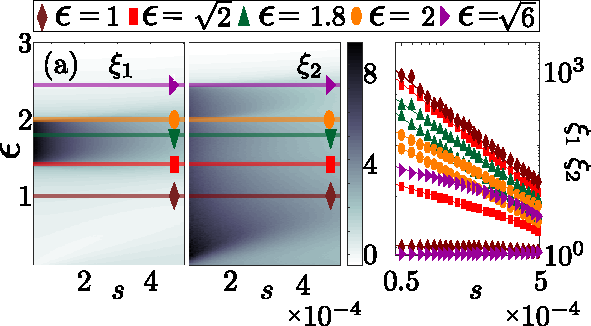
\includegraphics[width=0.5\textwidth]{graphics/loc_length_dipole_BW.pdf}

    \caption{\mm{We'll probably need a larger interval: a single order of magnitude is presumably not enough to adequately extract the scaling} (a) Localization lengths $\xi_1,\,\xi_2$ (color code)  as a function of the energy $\epsilon$ and the disorder strength $s \equiv \sigma / R_0$.
              The localization lengths along each of the solid lines are shown in loglog scale in panel (b) \mm{Is there a (b) in the panel? Have I got an old version of the figure?}. This allows us to extract the power law exponents $\nu$ characterizing the small-disorder behavior $\xi_i \sim s^\nu$.
              Grouping them by energy $\epsilon$, they read
                $\nu\left(\epsilon = 1\right)$ = \{ 0.1006~$\pm$~0.004, 1.96~$\pm$~0.03\}, 
 	        $\nu\left(\epsilon = \sqrt{2}\right)$ = \{ 0.823~$\pm$~0.006, 2.16~$\pm$~0.06\},
 		$\nu\left(\epsilon = 1.8\right)$ = \{ 1.986~$\pm$~0.007, 2.01~$\pm$~0.01\},   
  		$\nu\left(\epsilon = 2\right)$ = \{ 1.428~$\pm$~0.007, 1.376~$\pm$~0.007 \},
 		$\nu\left(\epsilon = \sqrt{6}\right)$ = \{ 0.034~$\pm$~0.002, 0.79~$\pm$~0.01 \}.
	 For these computations, the atomic position distribution is a Gaussian with width $\sigma$ \mm{what is the value of $R_0$?}, and the interatomic interaction is a dipole-dipole interaction ($\alpha = 3$) with an interaction strength of $V_0 = 300$.
	     } 
   \label{Fig:2D_loc_length}
\end{figure}  
%%%


First, we notice a slight bending of the features in panel (a) towards higher energies (i.e., down). This is due to the fact that the distribution of the $\delta V$s experiences a bias towards positive values, i.e., the energy shifts are preferentially positive, and this bias, for very small disorder, increases with $s$ (see \cite{SM}).
%%
Second, in panel (b) we display the scaling behavior of the localizatoin lengths $\xi_{1/2}$ as functions of $s$, which we analyze energy by energy in the table below: 
\begin{center}
\begin{tabular}{ | c || c | c |} \hline
   & $\nu$ from Ref.~\cite{Leykam2017} & $\nu$ from Fig.~\ref{Fig:2D_loc_length}(b) \\ 
   \hline \hline
 $\epsilon = 1$ & $(0,2)$ & $(0.1006 \pm ~0.004, 1.96 \pm 0.03)$ \\ \hline  
 $\epsilon = \sqrt{2}$ & $(2/3, 4/3)$ & $(0.823 \pm 0.006, 2.16 \pm 0.06)$  \\ \hline
 $\epsilon  = 1.8$ & $(2,2)$ & $(1.986 \pm 0.007, 2.01 \pm 0.01)$ \\ \hline
 $\epsilon = 2$ & $(2/3, 4/3)$ & $(1.428 \pm 0.007, 1.376 \pm 0.007)$ \\ \hline
 $\epsilon = \sqrt{6}$ & $(0, 2/3)$ & $(0.034 \pm 0.002, 0.79 \pm 0.01)$ \\
 \hline
\end{tabular}
\end{center}
\mm{I maintain that these errors seem unnaturally small} The usual scaling for Anderson localization corresponds to $\nu = 0$ at energies outside a band (``out''), $\nu = 2/3$ at a band edge (``edge'') and $\nu = 2$ inside a band (``in''). Matching the ordering of the localization lengths in the table, the chosen energies correspond to $\epsilon =1$ (out/in), $\sqrt{2}$ (edge, in), $1.8$ (in/in), $2$ (edge/in) and $\sqrt{6}$ (out/edge). The ``anomalous'' scaling $\nu = 4/3$ at $\epsilon = \sqrt{2}$ and $\sqrt{6}$ is attributed in Ref.~\cite{Leykam2017} to the coupling between the two detangled chains, which produces resonances between states in the middle of a band and states at the edge of the other one when the latter displays vanishing group velocity. Comparing these values with the ones we have found, we observe reasonable agreement at $\epsilon = 1$ and $\epsilon = 1.8$, for the anomalous scaling at $\epsilon = 2$ and for the ``out'' scaling at $\epsilon = \sqrt{6}$. The anomalous scaling at $\epsilon = \sqrt{2}$ seems instead to be ``cured'' as we retrieve a result compatible with the usual Anderson one ($\nu  \approx 2$), probably due to the ``alternating'' structure of the disorder, which in the detangled picture results in the absence of random couplings between $Y_n^{\pm}$ sites, present instead in \cite{Leykam2017}. The different scaling highlighted at the band edges (i.e., instead of $2/3$) at $\epsilon = \sqrt{2}$ and $2$ is difficult to explain at the moment. One important effect seems to be the aforementioned bias in the energy shifts: when approaching the band edges from inside (outside), in fact, the Anderson scaling $\nu = 2/3$ is modified to $\nu \approx 1$ ($1/2$). Clearly, however, this is not sufficient to fully account for the extracted values \mm{Is it possible to perform the same analysis for the reflected negative energies, which should display the opposite approach?}.

 








%%
%%---------------------------------------------------------------------------------------------------------------------------------------------------------------------------------------
%\section{Lieb ladder with correlated disorder}
%
%
%We observe a ``bending'' of the of the delocalized region of $\xi_1$ (Figure \ref{Fig:2D_loc_length}(a)) towards higher energies $\epsilon>2$, which does not occur for flat disorder.
%This bending is caused by the increase of the parameter $s$, which increases the disorder strength and changes the band structure of the disorder-free problem.
%
%
%
%
%%
%%\begin{figure}
%%
%%	      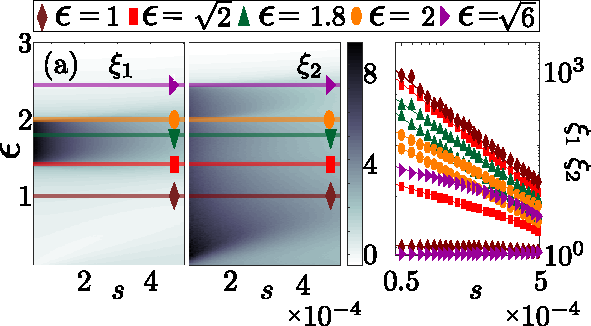
\includegraphics[width=0.5\textwidth]{graphics/loc_length_dipole_BW.pdf}
%%
%%    \caption{(a) Localization lengths $\xi_1,\,\xi_2$ (color code)  as a function of the energy $\epsilon$ and the disorder strength $s$.
%%              The localization lengths along each of the black lines are shown in (b).
%%              The power law exponents $\nu$ of $\xi_1,\,\xi_2$ are
%%                $\nu\left(\epsilon = 1\right)$ = \{ 0.1006~$\pm$~0.004, 1.96~$\pm$~0.03\}, 
%% 	        $\nu\left(\epsilon = \sqrt{2}\right)$ = \{ 0.823~$\pm$~0.006, 2.16~$\pm$~0.06\},
%% 		$\nu\left(\epsilon = 1.8\right)$ = \{ 1.986~$\pm$~0.007, 2.01~$\pm$~0.01\},   
%%  		$\nu\left(\epsilon = 2\right)$ = \{ 1.428~$\pm$~0.007, 1.376~$\pm$~0.007 \},
%% 		$\nu\left(\epsilon = \sqrt{6}\right)$ = \{ 0.034~$\pm$~0.002, 0.79~$\pm$~0.01 \}.
%%	 The atomic position distribution is a Gaussian with width $\sigma$, and the interatomic interaction is a dipole-dipole interaction ($\alpha = 3$) with an interaction strength of $V_0 = 300$.
%%	     } 
%%   \label{Fig:2D_loc_length}
%%\end{figure}  
%
%
%
%\subsubsection{discuss ``anomalous'' scaling presumably caused by correlations in disorder}
%Reference \cite{Leykam2017} gives the power law exponents for various energies
%%
%\footnote{Power law exponents \cite{Leykam2017}:
%$
%E = 1:\{\nu_{\xi_1} = 0,\nu_{\xi_2} = 2\}, E = \sqrt 2:\{\nu_{\xi_1} = 2/3,\nu_{\xi_2} = 4/3\},E = 1.8:\{\nu_{\xi_1} = 2,\nu_{\xi_2} = 2\},
%E = 2:\{\nu_{\xi_1} = 2/3,\nu_{\xi_2} = 4/3,E = \sqrt 6:\{\nu_{\xi_1} = 0,\nu_{\xi_2} = 2/3\}\}
%$.}
%for a Lieb ladder with a flat disorder 
%potential acting on all lattice sites, which we can reproduce in our setup where the (flat) disorder only acts on intermediate lattice sites.
%%
%When we apply the experimental disorder to our system, we find an anomalous scaling behavior of the localization lengths
%shown in Figure for $E = \sqrt{2}, 2$. In Fig \ref{Fig:2D_loc_length}, we fit the numerical data with the function $f(x) = a \cdot x^\nu$ to obtain the
%the power law exponents given in the caption.
%For $E = \sqrt 2$ the exponents $\nu_{\xi_1}\approx 1$ and  $\nu_{\xi_2}\approx 2$, while for $E = 2$, the localization lengths $\xi_1$ and $\xi_2$ are parallel (see orange curves) with a
%power law exponent $\nu_{\xi_1,\xi_2} \approx 3/2$.
%The energies $\epsilon = \sqrt 2, 2$, where the anomalous scaling appears, correspond to the situation where one of the dispersive channels has a band edge with zero group velocity,
%while the other dispersive channel 
%supports a mid-band state (Figure \ref{Fig:decoupling}(d)).
%The difference in the power law exponents between the flat and experimental disorder cannot be 
%associated with the fat-tails of the distribution of the $\delta V$, because 
%the probability of populating the tails of Eq. \eqref{eq:fattail} is, for the considered parameter regime, approximately zero.
%We checked that the anomalous scaling is not caused from the asymmetry of the distribution Eq. \eqref{eq:fattail} around the origin by calculating
%the localization length for a flat disorder of the $\delta_V$ which is not centered around the origin.
%Using a flat distribution on the atomic position, leading to correlated $\delta_V$, we obtain a very similar scaling behavior of the localization
%length shown in Figure \ref{Fig:2D_loc_length}(b).
















%
%---------------------------------------------------------------------------------------------------------------------------------------------------------------------------------------
\emph{Localized state dynamics---}
Reconstructing the localization lengths studied above in an experiment might be challenging. In particular accessing the large localization lengths would require sufficiently large system sizes. However, one can probe the influence of disorder by initializing the system in a specific state and tracking the subsequent dynamics by measuring the on-site excitation probabilities, which is done routinely in Rydberg quantum simulators [REFS].

Here, it is particularly interesting to investigate the dynamics of the localised states supported by the flatband which would not evolve if the disorder was absent. This provides a probe of many-body effects due to the disorder even for small system sizes. Lets consider the time evolution of the state $\ket{\psi_{\rm loc}} = 1/\sqrt{4} \left( A_i + B_i - E_i - E_{i+1} \right)$ localized at rungs $i,i+1$ of the ladder, see Fig. \ref{Fig:time evolution}a. The localized states can be in principle prepared by addressing lattice sites individually with laser pulses and exploiting both the facilitation and blockade condition \cite{SM}. We evolve $\ket{\psi_{\rm loc}}$ according to $H_{\rm eff}$ given by Eq. (\ref{eq:H eff}) \cite{SM}.


In the following we evaluate the probability of excitations $p^\alpha_i = n^\alpha_i/\sum_{i=1}^{L} n^\alpha_i$ at rung $i$. Here $n^\alpha_i = \bra{\psi(t)} \hat{n}^\alpha_i \ket{\psi(t)}$, $\alpha=u,l$ for the upper and lower leg of the ladder respectively and $\hat{n}^\alpha_i = \ket{S^\alpha_{i-1}}\bra{S^\alpha_{i-1}} + \ket{C_{i}}\bra{C_{i}} + \ket{S^\alpha_{i}}\bra{S^\alpha_{i}} + \ket{E_{i}}\bra{E_{i}}$ is the projector operator on all spin configurations which contain an excitation at rung $i$ and leg $\alpha$ with $S^u=A, S^l=B$.
%\begin{equation}
%	\hat{n}^\alpha_i =
%		\ket{S^\alpha_{i-1}}\bra{S^\alpha_{i-1}} + \ket{C_{i}}\bra{C_{i}} + \ket{S^\alpha_{i}}\bra{S^\alpha_{i}} + \ket{E_{i}}\bra{E_{i}}
%\end{equation}
%\begin{equation}
%	\hat{n}_i = 
%	\begin{cases}
%		\ket{A_{i-1}}\bra{A_{i-1}} + \ket{C_{i}}\bra{C_{i}} + \ket{A_{i}}\bra{A_{i}} + \ket{E_{i}}\bra{E_{i}} \\
%		\text{ upper leg} \\
%		\ket{B_{i-1}}\bra{B_{i-1}} + \ket{D_{i}}\bra{D_{i}} + \ket{B_{i}}\bra{B_{i}} + \ket{E_{i}}\bra{E_{i}} \\
%		\text{ lower leg}
%	\end{cases}
%\end{equation}
%is the projector operator on all spin configurations which contain an excitation at site $i$ and $S^u=A, S^l=B$. 
We then define the average position $\bar{x}$ and the standard deviation $\Delta x$ of the excitations as
\begin{eqnarray}
	\bar{x}^\alpha &=& \sum p^\alpha_i i \\
	\left( \Delta x^\alpha \right)^2 &=& \sum_i p^\alpha_i i^2 - \left(\bar{x}^\alpha \right)^2 = \sum_i p^\alpha_i (i-\bar{x}^\alpha)^2
	\label{eq:Delta x}
\end{eqnarray}

The results of the simulation are shown in Fig. \ref{Fig:time evolution} which shows the evolution of the initial spin excitation probabilities given by $\ket{\psi_{\rm loc}}$, Fig. \ref{Fig:time evolution}a, as a function of a dimensionless time $\tilde{t}=t \Omega$ for a specific value of the disorder strength $s=0.0014$ in Fig. \ref{Fig:time evolution}b. The standard deviation of the excitations $\Delta x$ as a function of $s$ is shown in Fig. \ref{Fig:time evolution}c for three different times. It can be seen that by increasing the disorder strength, the localized state becomes delocalized due to the coupling between the flat and the dispersive bands, causing their hybridization, \cite{Leykam2017}.

Increasing further the disorder, it results in large energy shifts which prevent hopping of the excitations under the facilitation condition and cause the state to localize again.

[{\bf Comment on what regime/disorder is achievable in the experiment? Should we try to come up with a specific example to give some numbers? Some extra work - not sure about the parameters for $1/r^3$ interactions.}]

\begin{figure}

	      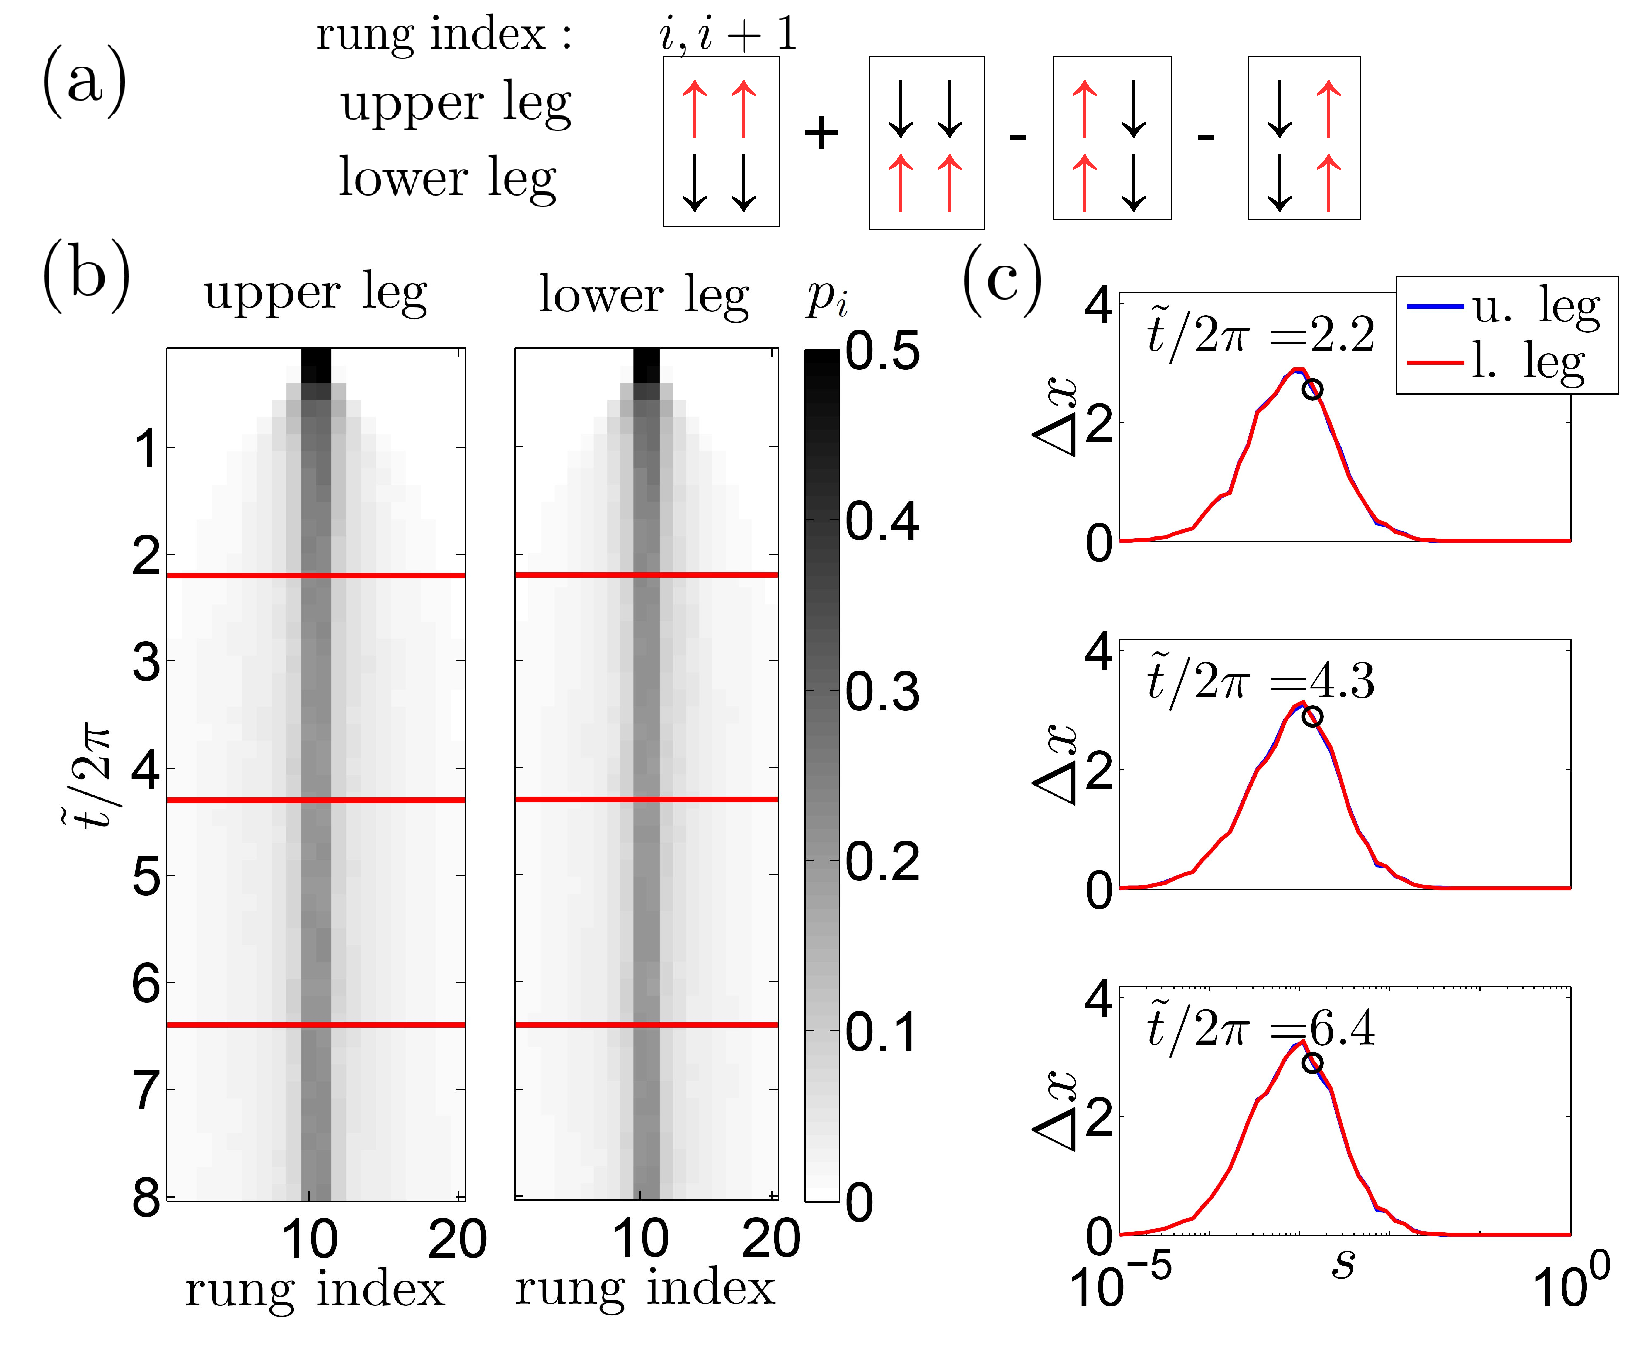
\includegraphics[width=0.5\textwidth]{graphics/time_evolution_CLS_PaperSupport_v4.pdf}
    %
		\caption{(a) Schematic representation of the spin configuration corresponding to the initial state $\ket{\psi_{\rm loc}}$ localized at rungs $i,i+1$ of the ladder. (b) The probability of excitations $p_i$ given by the time evolution of the localized state with an initial support in the middle (rungs 10 and 11) of the ladder of length 20 for $s=0.0014$. The left (right) pane shows the time evolution in the upper (lower) leg of the ladder. The horizontal red lines denote three different times for which the respective value of $\Delta x$ is shown as a black circle in (c). (c) Standard deviation of the excitation positions $\Delta x$ vs. the disorder strength $s$ for three different times. Blue (red) solid lines correspond to upper (lower) leg of the ladder respectively. Results obtained for 100 disorder realizations and $V_0/\Omega=200$.}

 \label{Fig:time evolution}
   
\end{figure}  

\emph{Conclusions and Outlook---} [{\bf FINISH!!}]

\emph{Acknowledgments---} [{\bf FINISH!!}]



%
%---------------------------------------------------------------------------------------------------------------------------------------------------------------------------------------
\section{Supplemental Material}


\subsection{Numerical simulation of the spin dynamics}

We consider the full Hamiltonian Eq. (\ref{Eq:Hamil_full}) which we rewrite as dimensionless quantity
\begin{equation}
	\tilde{H} = \sum_j \sigma_x^{(j)} + (-\tilde{V}(R_0)) n_j + \tilde{V}(R_0) \sum_{j>k} \frac{n_j n_k}{|j-k|^\alpha},
\end{equation}
where $\tilde{V}(R_0) = V(R_0)/\Omega$ (in what follows we label all dimensionless quantities by tilde). This leads to the following effective Hamiltonian on the Lieb lattice of length $L$ 
\begin{equation}
	H_{\rm eff} = H_0 \otimes \mathds{1}_L + H_0^{\rm dis} + \left[ H_1 \otimes G_L + {\rm H.c.} \right],
	\label{eq:H eff}
\end{equation}
expressed in the basis
\begin{equation}
	\mathcal{B}=\{A_1,..,A_L,B_1,..,E_L\},
	\label{eq:basis}
\end{equation}
where
\begin{equation}
	H_0 =
 \begin{pmatrix}
  	 0 & 0 & 1 & 0 & 0 \\
     0 & 0 & 0 & 1 & 0 \\
     1 & 0 & 0 & 0 & 1 \\
     0 & 1 & 0 & 0 & 1 \\
     0 & 0 & 1 & 1 & 0
 \end{pmatrix},
\end{equation}
$H_1$ is a $5 \times 5$ matrix with only non-zero entries $(H_1)_{1,3}=(H_1)_{2,4}=1$, $G_L = \delta_{i,i+1}$ is a $L \times L$ matrix with ones on the first upper diagonal and 
\begin{eqnarray}
	H_0^{\rm dis} = {\rm diag} & & \left( \tilde{\delta}_{A_1},...,\tilde{\delta}_{A_{L-1}},\tilde{\delta}_{A_{L}}=0, \right. \nonumber \\
									  & & \tilde{\delta}_{B_1},...,\tilde{\delta}_{B_{L-1}},\tilde{\delta}_{B_{L}}=0, \nonumber \\
									  & & \tilde{\delta}_{C_1}=0,...,\tilde{\delta}_{C_{L}}=0, \nonumber \\
									  & & \tilde{\delta}_{D_1}=0,...,\tilde{\delta}_{D_{L}}=0, \nonumber \\
									  & & \left. \tilde{\delta}_{E_1},...,\tilde{\delta}_{E_{L}} \right)
	\label{eq:disorder}
\end{eqnarray}
is a $5L \times 5L$ diagonal disorder matrix, where we impose open boundary conditions by requiring that $\tilde{\delta}_{A_L} = \tilde{\delta}_{B_L}=0$, since spin configurations corresponding to the $A_L,B_L$ basis elements are missing. Analogously we enforce the OBC in the coupling matrix by setting all Hamiltonian elements corresponding to the $L$-th and $2L$-th rows and columns to 0. Here, $\tilde{\delta}_{X_j} = \Omega \left(V(d_{X_j})-V(R_0) \right)$, where $X_j=A_j,..,E_j$ and $d_{X_j}$ is a shorthand for the spin separation in the given configuration $X_j$. We note that since configurations $C,D$ correspond to single spin excitation, the associated disorder is vanishing by definition, $\tilde{\delta}_{C_j} = \tilde{\delta}_{D_j} \; \forall j$. The disorder energies $\tilde{\delta}_{X_j}$ are generated from first drawing a specific realization of atomic positions at each site of the lattice in all three spatial directions with isotropic Gaussian distribution of width $s$.

We then exactly evolve an initial state
\begin{equation}
	\ket{\psi_0} = \sum_{j=1}^{5L} c_j \ket{b_j},
\end{equation}
as $\ket{\psi(t)} = {\rm exp}\left[ -i \tilde{t} H_{\rm eff}\right] \ket{\psi_0}$, where $b_j$ are the elements of the basis (\ref{eq:basis}) [strictly speaking there are only $5L-2$ non-trivial elements due to the OBC].

We note that the result of the evolution depends on two independent parameters, $s$ and the ratio $V(R_0)/\Omega$ which should satisfy...[{\bf link to the Supplement by Matteo/exemplify}] for the effective Hamiltonian (\ref{eq:H eff}) to be valid. In Fig. \ref{Fig:Dx_scan}a we present the results of the simulation analogous to that performed in Fig. \ref{Fig:time evolution}, showing $\Delta x$ in the $s - \Omega/V(R_0)$ plane. We observe that the maximum of $\Delta x$ as a function of the disorder gets shifted towards higher disorder as $\Omega$ is increased. 

First we note that in the dimensionless formulation, the off-diagonal hopping elements in $H_{\rm eff}$ are of a fixed amplitude 1. The dependence of $\Delta x$ in Fig. \ref{Fig:Dx_scan}a can be intuitively understood as follows. Smaller values of $\Omega/V(R_0)$ correspond to larger diagonal disorder elements $\tilde{\delta}$. Since it is the disorder which couples the flat and dispersive bands, the smaller the $s$, the smaller the $\Omega$ is sufficient to cause the excitation hopping and thus the increase in $\Delta x$. Similarly, when further increasing $s$, as soon as the corresponding disorder energies become dominant over $\Omega$, the hopping cannot overcome the energetic barriers and becomes inhibited, corresponding to the decrease in $\Delta x$. Clearly, by increasing $\Omega/V(R_0)$ higher values of $s$ are required to prevent the hopping. These two arguments, one for the increase and the other for the decrease of $\Delta x$ are then in agreement with the shift of the maximum $\Delta x$ from small to large values of $(s,\Omega/V(R_0)$ as shown in Fig. \ref{Fig:Dx_scan}a.

In Fig. \ref{Fig:Dx_scan}b,c we show a comparison between the exact evolution according to the full Hamiltonian (\ref{Eq:Hamil_full}), dashed line, and $H_{\rm eff}$, solid line. As expected, the predictions of the two models show an agreement in the regime where $\Omega \ll \delta V, V_{\rm NN}$ [{\bf unify notation!}], Fig. \ref{Fig:Dx_scan}c ($V(R_0)/\Omega=200$). On the other hand for larger $\Omega$, the two models start to differ as shown in Fig. \ref{Fig:Dx_scan}b ($V(R_0)/\Omega=20$). Due to the limited computational power, we have considered $L=4$ for the comparison between $H$ and $H_{\rm eff}$ instead of $L=20$ used in Fig. \ref{Fig:time evolution} and Fig. \ref{Fig:Dx_scan}a.


\begin{figure}

	      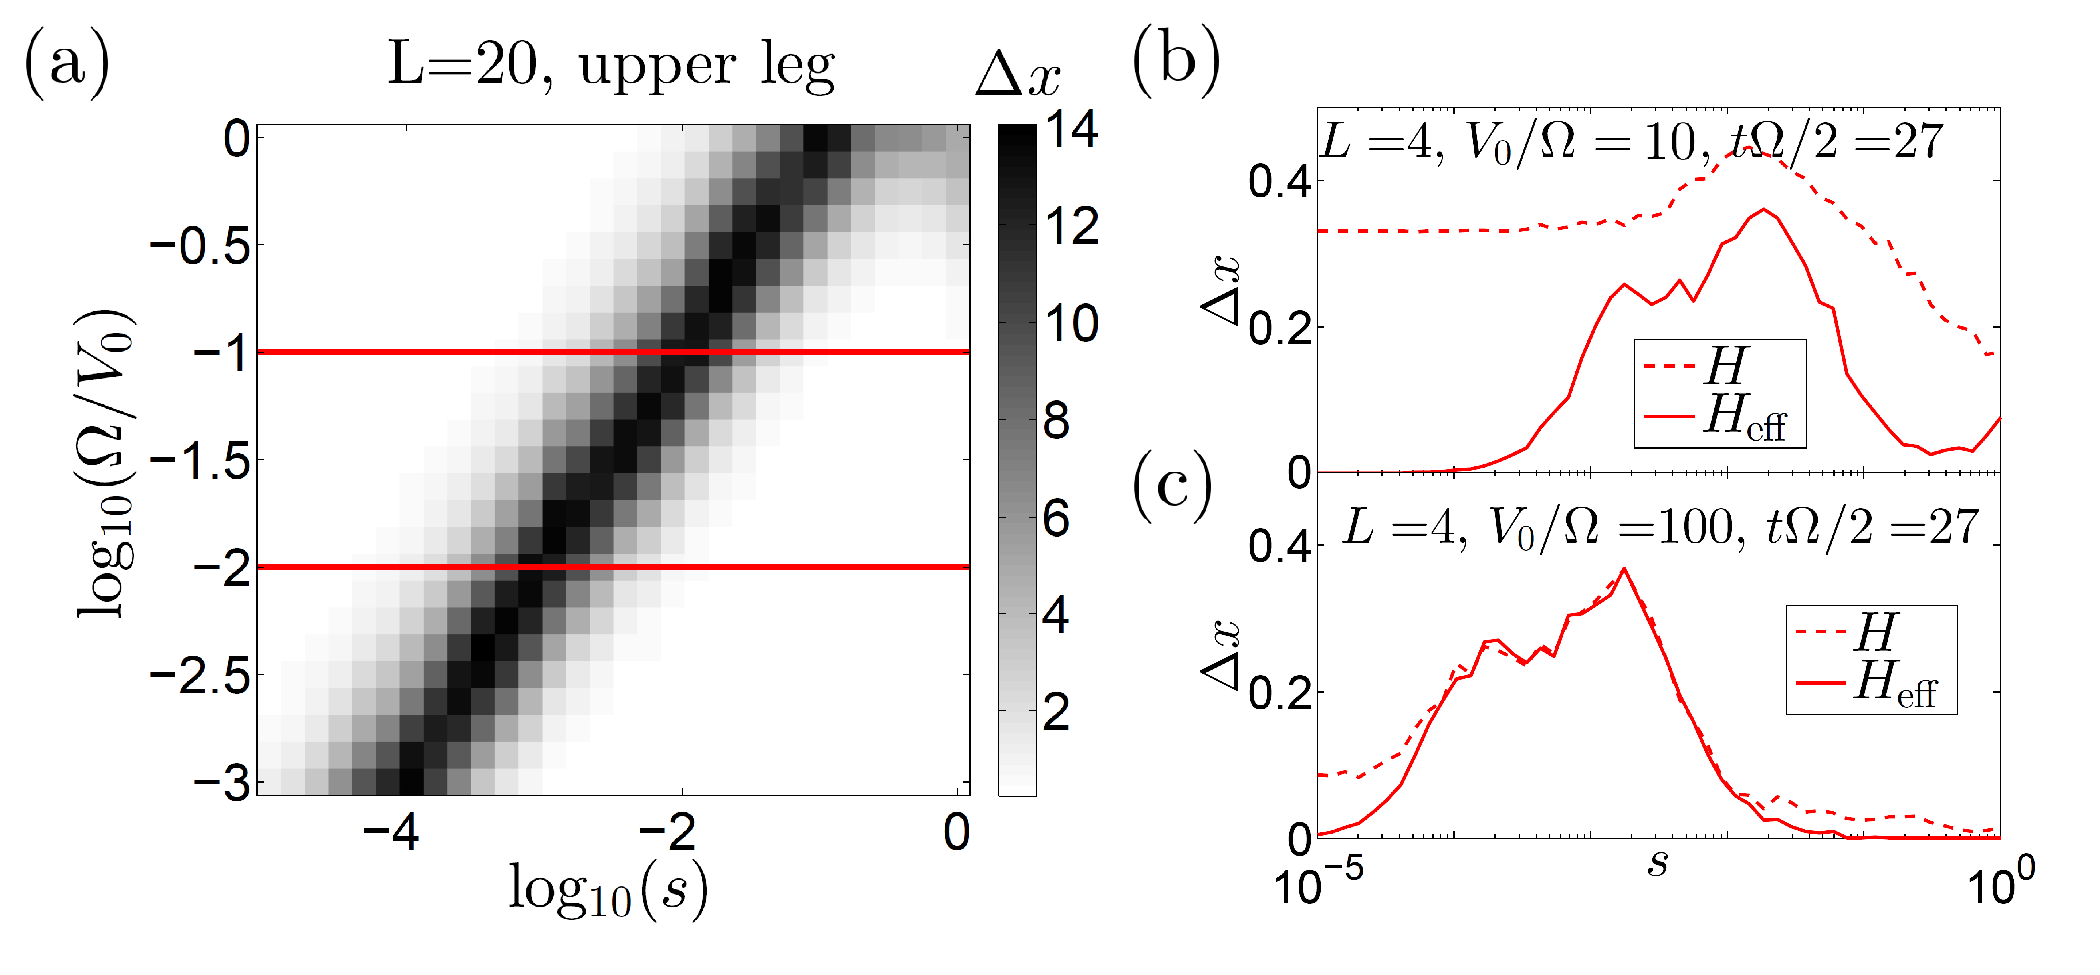
\includegraphics[width=0.5\textwidth]{graphics/Dx_vs_s_Omega.pdf}
    %
		\caption{[{\bf Correct for $\Omega$ vs. $\Omega/2$ !!!}](a) Standard deviation $\Delta x$, Eq. (\ref{eq:Delta x}), of the excitation positions in the $s-\Omega/V(R_0)$ plane. Here, $\Delta x$ was obtained by evolving the initial state $\ket{\psi_{\rm loc}}$ located at rungs 10 and 11 in the middle of the ladder of length $L=20$ by the effective Hamiltonian $H_{\rm eff}$. The two red solid lines correspond to a cut for fixed values of $\Omega/V(R_0)$, $\Omega/V(R_0)=1/10$ (upper line) and $\Omega/V(R_0)=1/100$ (lower line). (b) Comparison between the evolution of $\ket{\psi_{\rm loc}}$ generated by $H$, Eq. (\ref{Eq:Hamil_full}), dashed line and $H_{\rm eff}$, solid line in a ladder of $L=4$ and for $\Omega/V(R_0)=1/10$. (c) Same as (b) with $\Omega/V(R_0)=1/100$. Here we have used $\tilde{t}/2 \pi = 4.3$ for each respective $\Omega'$ and averaged over 100 disorder realizations. 
		}
 \label{Fig:Dx_scan}
   
\end{figure}  


\subsection{Initial state preparation}


Lets consider the preparation of the state $\ket{\psi_{\rm loc}} = 1/\sqrt{4} \left( A_i + B_i - E_i - E_{i+1} \right)$ localized at rungs $i,i+1$ of the ladder. The state $\ket{\psi_{\rm loc}}$ can then be obtained by application of five pulses on initially all atoms in the spin-down state as $\ket{\psi_{\rm loc}} = \mathcal{B}_1(2 \pi) \mathcal{F}_3(\pi) \mathcal{F}_2(\frac{\pi}{2}) \mathcal{B}_4(\pi) \mathcal{B}_1(\frac{\pi}{2}) \ket{\psi_{\downarrow..\downarrow}}$, where $\mathcal{B}_j(\theta),\mathcal{F}_j(\theta)$ stand for the laser pulse of area $\theta$ in the blockaded ($\mathcal{B}$) and facilitated ($\mathcal{F}$) regime applied at site $j=1,..,4$ labeling the effective plaquette formed by the four sites corresponding to the $i$-th and $(i+1)$-th rung of the ladder, see Eq. (\ref{eq:preparation}). [{\bf Correct and Finish!!}]

\begin{eqnarray}
%
\boxed{
\begin{matrix}
  \downarrow_1 & \downarrow_2 \\
  \downarrow_3 & \downarrow_4
 \end{matrix}
}
% ***************************************************
	& \xrightarrow[]{\mathcal{B}_1(\frac{\pi}{2})} &
-i \, \boxed{
\begin{matrix}
  {\color{red} \uparrow} & \downarrow \\
  \downarrow & \downarrow
 \end{matrix}
}
+
\boxed{
\begin{matrix}
  \downarrow & \downarrow \\
  \downarrow & \downarrow
 \end{matrix}
} 
\nonumber \\
%======================================================================
	& \xrightarrow[]{\mathcal{B}_4(\pi)} &
\phantom{-i \,} \boxed{
\begin{matrix}
  {\color{red} \uparrow} & \downarrow \\
  \downarrow & \downarrow
 \end{matrix}
}
+
\boxed{
\begin{matrix}
  \downarrow & \downarrow \\
  \downarrow & {\color{red} \uparrow}
 \end{matrix}
} 
\nonumber \\
%======================================================================
	& \xrightarrow[]{\mathcal{F}_2(\frac{\pi}{2})} &
-i\,\boxed{
\begin{matrix}
  {\color{red} \uparrow} & {\color{red} \uparrow} \\
  \downarrow & \downarrow
 \end{matrix}
}
+
\boxed{
\begin{matrix}
  {\color{red} \uparrow} & \downarrow \\
  \downarrow & \downarrow
 \end{matrix}
}
-i\,\boxed{
\begin{matrix}
  \downarrow & {\color{red} \uparrow} \\
  \downarrow & {\color{red} \uparrow}
 \end{matrix}
}
+
\boxed{
\begin{matrix}
  \downarrow & \downarrow \\
  \downarrow & {\color{red} \uparrow}
 \end{matrix}
} 
\nonumber \\
%======================================================================
	& \xrightarrow[]{\mathcal{F}_3(\pi)} &
\phantom{-i \,}\boxed{
\begin{matrix}
  {\color{red} \uparrow} & {\color{red} \uparrow} \\
  \downarrow & \downarrow
 \end{matrix}
}
+
\boxed{
\begin{matrix}
  {\color{red} \uparrow} & \downarrow \\
  {\color{red} \uparrow} & \downarrow
 \end{matrix}
}
+
\boxed{
\begin{matrix}
  \downarrow & {\color{red} \uparrow} \\
  \downarrow & {\color{red} \uparrow}
 \end{matrix}
}
+
\boxed{
\begin{matrix}
  \downarrow & \downarrow \\
  {\color{red} \uparrow} & {\color{red} \uparrow}
 \end{matrix}
} 
\nonumber \\
%======================================================================
	& \xrightarrow[]{\mathcal{F}_4(2\pi)} &
\phantom{-i \,}\boxed{
\begin{matrix}
  {\color{red} \uparrow} & {\color{red} \uparrow} \\
  \downarrow & \downarrow
 \end{matrix}
}
+
\boxed{
\begin{matrix}
  {\color{red} \uparrow} & \downarrow \\
  {\color{red} \uparrow} & \downarrow
 \end{matrix}
}
-
\boxed{
\begin{matrix}
  \downarrow & {\color{red} \uparrow} \\
  \downarrow & {\color{red} \uparrow}
 \end{matrix}
}
-
\boxed{
\begin{matrix}
  \downarrow & \downarrow \\
  {\color{red} \uparrow} & {\color{red} \uparrow}
 \end{matrix}
} 
\nonumber \\
%======================================================================
	& \xrightarrow[]{\mathcal{F}_2(2\pi)} &
\phantom{-i \,}\boxed{
\begin{matrix}
  {\color{red} \uparrow} & {\color{red} \uparrow} \\
  \downarrow & \downarrow
 \end{matrix}
}
-
\boxed{
\begin{matrix}
  {\color{red} \uparrow} & \downarrow \\
  {\color{red} \uparrow} & \downarrow
 \end{matrix}
}
-
\boxed{
\begin{matrix}
  \downarrow & {\color{red} \uparrow} \\
  \downarrow & {\color{red} \uparrow}
 \end{matrix}
}
+
\boxed{
\begin{matrix}
  \downarrow & \downarrow \\
  {\color{red} \uparrow} & {\color{red} \uparrow}
 \end{matrix}
} \nonumber \\
%
\label{eq:preparation}
\end{eqnarray}



\subsection{Transfer Matrix [TO BE EDITED]}

The values $\xi_{1/2}$ are found via a transfer matrix formalism: we start by writing a generic state of the system as 
\be
\begin{split}
	\ket{\psi} = \sum_n \lqq  X_n^+ \ket{X_n^+} + X_n^- \ket{X_n^-} + \right. \\
	\left. + Y_n^+ \ket{Y_n^+} + Y_n^- \ket{Y_n^-} + E_n \ket{E_n}    \rqq,
\end{split}
\ee
where $\ket{(\cdot)_n}$ denotes the state corresponding to the site labelled by $(\cdot)_n$, whereas we write simply $(\cdot)_n$ for the corresponding coefficient. The Schr\"odinger equation $H \ket{\psi} = \epsilon \ket{\psi}$ can now be recast in a matrix-vector product form for the four amplitudes $\psi_n = (X_n^+, X_n^-, Y_n^+, Y_n^-)^\intercal$ \cite{SM} which reads $\psi_{n+1} = T_{XY,n} \psi_n$. The transfer matrix $T_{XY,n}$ reads
%
  \begin{align}
    \begin{pmatrix} 
	\gamma_n \alpha_n  -1        &   \gamma_n \delta_{X^-_n}                & -\gamma_n         & 0 \\
	  -\epsilon \delta_{X^-_n}          & \epsilon \alpha_n  -1              & 0      & -\epsilon \\
	  \alpha_n                                & -\delta_{X^-_n}                                          & -1              & 0\\
	    -\delta_{X^-_n}                                 &  \alpha_n                                        &  0              & -1        
  \end{pmatrix}
  \label{Eq:Transfer_Matrix}
  \end{align}
 where $\gamma = \epsilon - \tfrac{2}{\epsilon-\delta_{E_{n+1}}}$, $\alpha_n = \epsilon - \delta_{X^+_n}$, and we introduced the shorthand $\delta_{E_n} = \delta V_{E_n}$, $\delta_{X_n^\pm} = \delta V_{A_n} \pm \delta V_{B_n}$. The operator norm of the product of $N$ of these matrices will generically grow as $\rme{N / \xi_1}$; a careful analysis can then highlight the subleading contributions \cite{a_Dwivedi_PRB_93} and allow one to extract a behavior $\sim \rme{N / \xi_2}$ as well, permitting the extraction of the localization lengths. The result is displayed in Fig.~\ref{Fig:2D_loc_length} which shows $\xi_1$ and $\xi_2$ as a function of the energy $\epsilon$ and the amplitude of the noise, quantified by $s \equiv \sigma / R_0$. 


\bibliographystyle{apsrev4-1}

\bibliography{bibliography}


\end{document}